%!TEX root = ../Main.tex

\chapter{Exercise 3.4}
\textbf{Create a cycle accurate communication model of a master and slave module that uses the
Avalon Streaming Bus interface (ST). Simulate that a master are transmitting data to a slave
module as illustrated in the figures 5-2 and 5-8. The slave should store received data from the master
in a text file. Include in the model a situation where the data sink signals ready = ‘0’. The simulated result
should be presented in the GTK wave viewer, so a VCD trace file must be created. It should be
possible to configure the channel, error and data size define in a separate header file as illustrated
in the below code snippet.}


A total of of three .h files and 4 .cpp files have been made in this exercise. A Master.h, Slave.h and Top.h with corresponding .cpp files. A main.cpp has also been made. 

The code below shows the Master.cpp code. The comments explain how the code works, but the essence of it is just to send an integer(1) and afterwards increment that integer for the next send cycle. That means the master will send the numbers 1...10. The master and slave are setup to use the Avalon Streaming Bus interface. The data transfer uses backpressure with a ready latency set to 1.  



\begin{lstlisting}
void Master::MasterThread(void)
{
	//Arbitrary data to send.
	dataToSend = 1;
	while (1)
	{
		// Update ready state - Will not be updated until next clock cycle.
		readyState = ready.read();
		
		// Check if slave is ready to receive data
		if (readyState)
		{
			// Indicate that data is being written
			valid.write(true);
			
			// Write data
			data.write(dataToSend);
			
			//Change data
			dataToSend += 1;
			
			// Set channel to 1
			channel.write(1);
			
			// set error to 0
			error.write(0);
		}
		else
		{
			// Indicate that no data is being written
			valid.write(false);
			
			// Write 0 to data (only to prettify in GTK-viewer).
			data.write(0);
			
			// Set channel to 0
			channel.write(0);
			
			// set error to 1
			error.write(1);
		}
		
		// Wait until next clock cycle.
		wait();
	}
}
\end{lstlisting}

The slave.cpp can be seen below. Again the comments explains how the code works. Whenever the slave has received 10 integers from the master, it begins to print those numbers to a text file. The slave also changes it's ready state every three clock cycle.  

\begin{lstlisting}
void Slave::SlaveThread(void)
{
	// Initial state of "ready".
	ready.write(false);
	
	// Simulate ready going low for 3 cycles, then high for 3 cycles, etc..
	while (1)
	{
		// read new data if any valid data
		if (valid.read())
		{
			test_data = data.read();
			test_data_array[array_index] = test_data;
			array_index++;
			cout << "Slave received data: " << test_data << endl;
			
			// Print the first 10 numbers recieved by the slave to a text file
			if (test_data_array[9] != 0)
			{
				ofstream myfile("Slave_data.txt");
				if (myfile.is_open())
				{
					for (int i = 0; i <= 9; i++)
					{
						myfile << test_data_array[i] << "\n";
					}
					
					myfile.close();
				}
				else cout << "Unable to open file";
			}
		}
		
		// Make sure that slave is ready for 3 cycles, then not ready for 3 cycles.
		if (state_counter < 3)
		{
			ready.write(true);
		}
		else
		{
			ready.write(false);
		}
		state_counter++;
		state_counter = state_counter % 6;
		
		wait(clk.posedge_event());
	}
}
\end{lstlisting}

In the Top.cpp file the different modules are being connected to each other using signal variables. It is also here the tracefile is made. A screenshot of the tracefile can be seen below.

\begin{figure}[H]
	\centering
	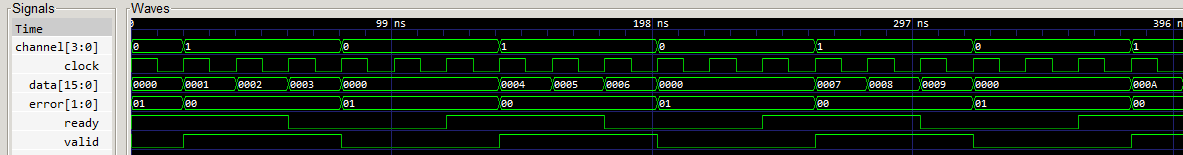
\includegraphics[width=\textwidth]{Images/GTK_3_4.png}
	\caption{A screenshot of GTK viewer}
	\label{fig:GTK_Viewer}
\end{figure}

According to the figure above we can confirm that the protocol is acting as it should.
